\section{Розробка пакету fastLBP}\label{section2.2}

Працюючи в лабораторії системної біології SysBio Інституту молекулярної біології та генетики під керівництвом А.О. Фролової 
та у колаборації із університетом Sanger було розроблено програмне забезпечення для ефективного обчислення гістограм 
рівномірних текстурних дескрипторів LBP.
ПЗ оформлено у вигляді пакету Python і доступне публічно через PyPi як \href{https://pypi.org/project/fastlbp-imbg/}{fastlbp-imbg}.
Вихідний код опубліковано у репозиторії \url{https://github.com/imbg-ua/fastLBP} на Github.

\subsection{Опис функціональності}\label{section2.2a}\hfill

Пакет складається з двох принципових частин. 
Перша частина -- це оптимізований код обчислення рівномірних LBP дескрипторів на мові Cython, що компілюється у бінарний модуль Python 
і доступний ззовні як функції \verb|fastlbp_imbg.lbp.uniform_lbp_uint8|, \verb|uniform_lbp_uint8_masked| та подібні.
Модуль розроблено на основі реалізації у пакеті Scikit-Image (\verb|skimage.feature.local_binary_pattern|).
Головними перевагами модуля є в декілька разів менше використання пам'яті, дещо швидше обчислення, і підтримка маскування вхідного масиву для 
пропуску частини пікселів.

Друга частина пакету це багатопотокова утиліта обчислення локальних ознак (гістограм) на основі рівномірних LBP дескрипторів із різними параметрами $R$ та $P$.
Ознаки обчислюються для неперетинних патчів зображення визначеного розміру як конкатенація гістограм.
Багатопотоковість дає можливість у рази зменшити час обчислення у середовищах із достатньою кількістю процесорів.
Утиліта адаптована для особливостей роботи із великими зображеннями: 
передбачено зберігання проміжних результатів, оптимізовано операції введення-виведення, 
реалізовано кешування для того, щоб уникнути повтору деяких проміжних обчислень.

\subsection{Особливості реалізації дескриптора}\label{section2.2b}\hfill

У реалізації дескриптора в fastLBP підтримується лише рівномірний варіант LBP.
Це дозволило спеціалізувати функцію обчислення LBP коду, позбавитись багатьох перевірок у головному циклі, і уточнити типи даних для вхідних та вихідних масивів.
Основне зменшення використання пам'яті походить від використання \verb|uint16| замість стандартних \verb|float64|, 
і уникнення зайвих копіювань даних у Python-обгортці основної функції.

Для випадків, коли необхідно обчислити ознаки лише частини зображення, розроблено масковані варіанти дескриптора. 
Функція \verb|uniform_lbp_uint8_patch_masked| приймає бінарну маску патчів, які потрібно обчислити, що дозволяє пропускати обчислення пікселів цілими блоками. 

\subsection{Особливості реалізації утиліти обчислення ознак}\label{section2.2c}\hfill

Обчислення ознак розділено на підзадачі за каналами та параметрами $R,P$ і відбувається у декілька етапів.
Спершу для фіксованих $(R,P)$ обчислюються LBP коди фіксованого каналу зображення (або на маскованих частинах зображення).
Далі зображення розділюється на патчі однакового визначеного розміру і обчислюється гістограма значень дескриптора для кожного патча.
Результати записуються у попередньо визначений сегмент файлу на диску.
Структура файлу визначена так, що після запису всіх сегментів утворюється масив конкатенованих гістограм, по одній для кожного патча зображення.
Таким чином ознака патча утворюється як конкатенація гістограм $H_1,\dots ,H_r$ LBP дескрипторів із параметрами $(R_1,P_1),\dots ,(R_r,P_r)$ для кожного каналу зображення 
(спершу всі гістограми одного каналу, потім наступного, і так далі).
Ці ознаки далі успішно використовувалися у задачах сегментації зображення.

Розміри патча можуть бути як більше, так і менше за $R$.
Важливо, що для коректного обчислення гістограм, недостатньо лише пікселів патча: 
для обчислення LBP кодів пікселів, близьких до межі, необхідні значення пікселів сусідніх патчів.

Для зручності роботи реалізовано кеш значень дескрипторів. 
Це дозволяє пробувати різні версії ознак без потреби обчислювати всі значення дескриптора заново, 
а також допомагає в роботі із великими зображеннями -- обчислення не втрачаються повністю за аварійного переривання роботи утиліти.

\begin{figure}[h]
    \centering
    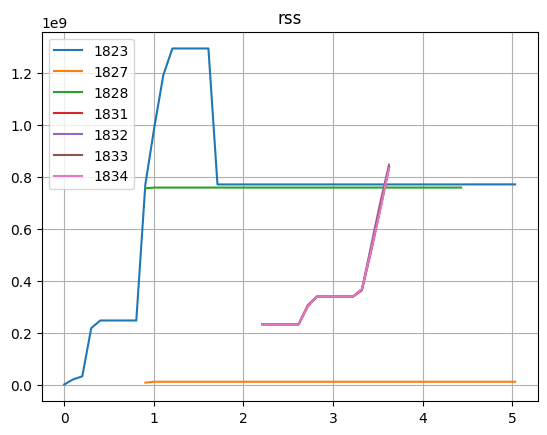
\includegraphics[width=0.5\textwidth]{img/fastlbp/memtest-1-rss.png}
    \caption{
        Типовий профіль використання пам'яті різними підпроцесами утиліти.
    }
    \label{fig:memprofile}
\end{figure}

Впродовж розробки утиліти приділено багато часу оптимізації швидкодії та використання пам'яті. 
На рис.~\ref{fig:memprofile} зображено типовий профіль використання пам'яті підпроцесами.
Особливо виділяються синій материнський процес, що виконує підготовчу роботу і запускає інші; 
та родина дочірніх процесів із поступово зростаючим споживанням.
Поширеними причинами великого споживання пам'яті було некоректне розміщення масивів у пам'яті перед передачею дочірнім процесам 
та копіювання масивів, яке можна уникнути. 

Через багатопотокове обчислення, підбір метрик використання пам'яті та інших метрик ефективності виявився неочевидною задачею.
Також, швидкодія і використання пам'яті багатогранно перевірялися у реальних умовах на обчислювальному кластері Sanger.
Окрім цього, вся ключова функціональність пакету перевіряється автоматичним тестуванням -- від коректності обчислення дескрипторів та очікуваного впливу параметрів обчислення ознак, 
до перевірки дрібних допоміжних функцій і роботи з файловою системою. 

Утиліта стала частиною більшого алгоритму сегментації гістопатологічних зображень, 
представленого на конференції ECCB 2024 \cite{fastlbp2024}.

\subsection{Оцінка швидкодії}\label{section2.2d}\hfill

Було виконано багатостороннє тестування пакету і оцінка його часу виконання й використання пам'яті, 
а також оцінка залежності цих величин від вхідних параметрів.
Практично підтверджено, що час виконання лінійно залежить від кількості пікселів у зображенні (рис.~\ref{subfig:time-vs-npixels}), 
що вказує на коректність реалізації. Доведено ефективність паралелізації обчислень у певному діапазоні кількості процесорів (рис.~\ref{subfig:parallell-efficiency-a}, рис.~\ref{subfig:parallell-efficiency-b}),
та доцільність використання маски для пропуску частин зображення (рис.~\ref{subfig:parallell-efficiency-с}).
Для надійності, кожен тест швидкодії виконувався декілька разів. На графіку точка вказує на медіану виміряної величини, 
а вертикальний відрізок навколо точки показує розкид між мінімальним та максимальним значеннями.

\begin{figure}[h]
    \begin{subfigure}{0.45\textwidth}
    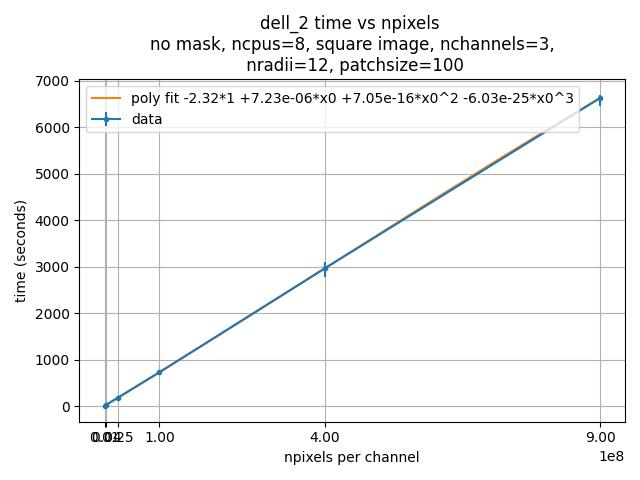
\includegraphics[width=0.99\linewidth]{img/fastlbp/complexity-time_npixels_nc3.jpg}
    \caption{
        Час виконання fastLBP від кількості пікселів.
    }
    \label{subfig:time-vs-npixels}
    \end{subfigure}%
    \begin{subfigure}{0.45\textwidth}
    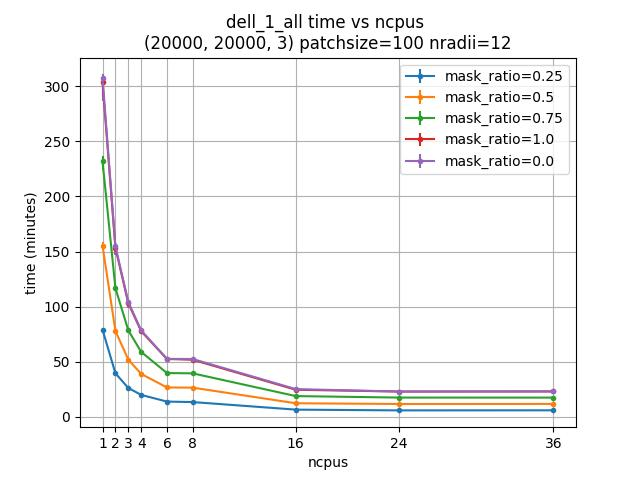
\includegraphics[width=0.99\linewidth]{img/fastlbp/time_ncpus.jpg} 
    \caption{
        Час виконання від кількості процесорів для масок різної площі.
    }
    \label{subfig:parallell-efficiency-a}
    \end{subfigure}

    \begin{subfigure}{0.45\textwidth}
    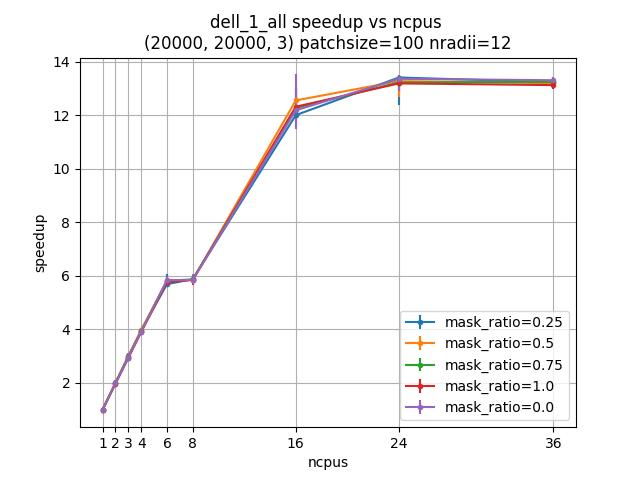
\includegraphics[width=0.99\linewidth]{img/fastlbp/speedup_ncpus.jpg}
    \caption{
        Пришвидшення від кількості процесорів для масок різної площі.
    }
    \label{subfig:parallell-efficiency-b}
    \end{subfigure}%
    \begin{subfigure}{0.45\textwidth}
    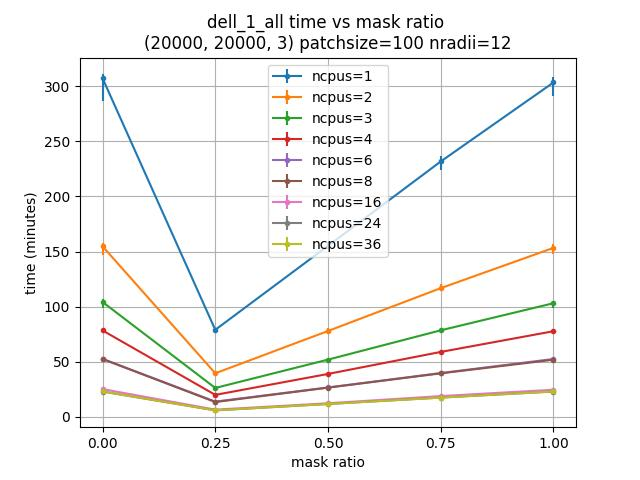
\includegraphics[width=0.99\linewidth]{img/fastlbp/time_mr.jpg}
    \caption{
        Час від площі маски для різних кількостей процесорів.
    }
    \label{subfig:parallell-efficiency-с}
    \end{subfigure}
    
    \caption{Результати оцінки швидкодії.}
    \label{fig:parallell-efficiency}
\end{figure}